%% Load document class fithesis2
%% {10pt, 11pt, 12pt}
%% {draft, final}
%% {oneside, twoside}
%% {onecolumn, twocolumn}
\documentclass[12pt,final,oneside]{fithesis2}

%% Basic packages
\usepackage[english]{babel}
\usepackage{cmap}
\usepackage[T1]{fontenc}
\usepackage{lmodern}
\usepackage[utf8]{inputenc}
\usepackage{graphicx}

%% Additional packages for colors, advanced
%% formatting options, etc.
%\usepackage{color}
%\usepackage{microtype}
%\usepackage{url}
%\usepackage{cslatexquotes}
%\usepackage{fancyvrb}
%\usepackage[small,bf]{caption}
\usepackage[plainpages=false,pdfpagelabels,unicode]{hyperref}
%\usepackage[all]{hypcap}

\usepackage{amsmath}
\usepackage{listings}

\lstset{
    basicstyle=\small\ttfamily,
    captionpos=b
}

\usepackage{tikz}

\newcommand\emptypage{\newpage\null\thispagestyle{empty}\newpage}

\setcounter{tocdepth}{3}

%% Fix long URLs in DVIs
%\usepackage{ifpdf}

%\ifpdf
%\else
%  \usepackage{breakurl}
%\fi

%% Packages used to generate various lists
%\usepackage{makeidx}
%\makeindex

%\usepackage[xindy]{glossaries}
%\makeglossary

%% Use STAR and CIRCLE signs for nested
%% itemized lists
%\renewcommand{\labelitemii}{$\star$}
%\renewcommand{\labelitemiii}{$\circ$}

%% Title page information
\thesistitle{String abstract domains}
\thesissubtitle{Master's thesis}
\thesisstudent{Bc. Matej Šuta}
\thesiswoman{false} %% Important when using Slovak or Czech lang
\thesisfaculty{fi}  %% {fi, eco, law, sci, fsps, phil, ped, med, fss}
\thesislang{en}     %% {en, sk, cs}
\thesisyear{Spring 2013}
\thesisadvisor{Mgr. Karel Klíč}

%% Beginning of the document
\begin{document}

%% Front page with a logo and basic thesis information
\FrontMatter
\ThesisTitlePage

\emptypage

%% Thesis declaration (required)
\begin{ThesisDeclaration}
  \DeclarationText
  \AdvisorName
\end{ThesisDeclaration}

%% Thanks (optional)
\begin{ThesisThanks}
My thanks go to ...
\end{ThesisThanks}

%% Abstract (required)
\begin{ThesisAbstract}
This thesis is about ...
\end{ThesisAbstract}

%% Keywords (required)
\begin{ThesisKeyWords}
static analysis, abstract interpretation, abstract domain, string,
prefix, suffix, trie
\end{ThesisKeyWords}

%% Beginning of the thesis itself
\MainMatter

%% TOC (required)
\tableofcontents


\chapter{Introduction}

Computers have followed Moore's~law~\cite{Moore65-1} for more than
four decades now. Hardware gets more powerful and complex. Consequently,
this results in software being more complex too. It has to be designed
with maintainability and reliability in mind. Therefore several software
verification methods have been created. Abstract interpretation is one
of them.

There are many aspects of a computer program that may be analyzed by
abstract interpretation. The focus of this thesis is
is how program manipulates strings. A string is very flexible data
structure that allows programmer to represent practically anything.
In fact, most of the programs written today have to deal with strings
in some form. Thus, it is important to know how programs treat strings.

This thesis describes string abstract domains in context of abstract
interpretation framework. It is based on papers published
by Cousot~\cite{CousotCousot77-1} and other authors. The goal of the thesis
is to design, implement and integrate several abstract domains for strings
into \texttt{canal} abstract interpreter. \texttt{canal} is a tool designed
to analyze behavior of application programs written in \texttt{C}.

The text has the following outline: chapter~\ref{chap:preliminaries}
presents preliminaries required to understand the abstract interpretation.
In chapter~\ref{chap:design} several string abstract domains are designed.
The implementation of designed domains is described in great detail in
chapter~\ref{chap:implementation}. Finally, thesis findings are summarized
in chapter~\ref{chap:conclusion}. Appendix~\ref{chap:instructions} contains
instructions for compiling and running the \texttt{canal} abstract
interpreter.


\chapter{Static analysis and abstract interpretation}
\label{chap:preliminaries}

The notion of quality is an abstract concept. In software engineering it
represents a multi-aspect property of a product which includes but is not
limited to characteristics such asstability, maintainability, realiability,
efficiency or security. It plays an important role in recognition of
particular software.

It is certainly true that not every project needs to have as high quality as
safety critical systems but to a certain degree quality matters
everywhere. It is crucial for software maintainability which becomes
especially difficult when size of a codebase and number of developers
increases. This chapter describes various techniques used to
improve these properties and abstract interpretation in particular.


\section{Software quality evaluation techniques}

Traditionally the set of quality control techniques are referred to as
validation and verification. According to
Boulanger~\cite{Boulanger12-1} these terms are defined in standard
ISO 9000:2000 as:

\begin{description}

\item[Verification] \hfill \\
confirmation by tangible proof that the specified requirements have
been met at each stage of the realization process

\item[Validation] \hfill \\
confirmation by tangible proof that the requirements for a specific use or
an anticipated application have been met

\end{description}

Applied in software engineering the definitions above summarize the
processes that ensure and demonstrate that the resulting software product
achieves the desired quality level.

The validation is usually performed by executing a program with intention
to assure that the software product meets the requirements of a customer.
The process can be manual or completely automatic. It includes
various types of tests such as acceptance testing, performance testing,
penetration testing, etc. Functional testing consists of test cases
being executed to check various scenarios and is traditionally performed
by quality assurence specialist. Main benefit of testing is that the
application is run under real confitions and the specialist is able to
check the presence of yet unidentified errors. The output of the validation
is statement whether the built solution is the right one.

The verification may be done either by executing the program or by
analyzing the source code of the program. They are called \textit{dynamic} 
and \textit{static} verification respectively. These activities are
typically performed by a programmer during the development phase.
There are many disciplines that enforce the verification by program
execution -- unit testing or integration testing among others. These
disciplines are relatively easy to understand and implement. The main
disadvantages include testing in isolation. In addition, this type of
testing can only check for presence of known errors. The static
verification usually includes source code inspection either manually or
by a tool. Implementation of such tool usually requires a deep
theoretical knowledge and programming skills.

Note that it is possible for program to pass the verification and
fail the validation step, hence the realationship between the approaches
should complementary rather then contradictory in order to achieve the
highest possible quality. Moreover, there is no
precise distinction between the two. Test driven development or behavior
driven development are two examples of techniques which perform
verification by executing unit tests and also validate that requirements
have been met.


\section{Static analysis}

Static code analysis is a well known term in software industry yet there
is a lot of confusion surrounding it. Emanuelsson and Nilsson
\cite{EmanuelssonNilsson08-1} refer to it as the analysis of a computer
program without actually executing it. This process is fully automatic
but a programmer needs to interpret the results of analysis and make
proper adjustments to the analyzed code.

Most of the languages do not have a support for runtime error detection.
It is programmers responsibility to ensure these errors do not occur
and deal with them once they do. The errors do not include simple type
checking or syntax errors although even these could be considered a part
of static analysis. They are already checked by compiler. Hence, only
errors which lead to unexpected or undefined behavior are checked.
Consider the \texttt{C} code in listing~\ref{lst:outofbounds}:

\begin{lstlisting}[
    language=C,
    caption={Out of bounds array access},
    label=lst:outofbounds
]

    int array[3] = { 1, 2, 3 };
    int value = array[3];

\end{lstlisting}

In the example the \texttt{array} variable contains three integers but
\texttt{value} variable will contain unexpected value because it is
accessing the fourth element of the \texttt{array}. Moreover, the
listing will compile and run, but the number might be different every
time the program is run since accessing the items out of array bounds is
undefined behavior in \texttt{C} programming language. Other typical
examples of errors potentially detected by static analysis could be
division by zero or infinite loops.

The applications of static analysis are quite extensive as it has been
shown by Emanuelsson and Nilsson \cite{EmanuelssonNilsson08-1}. Besides
already mentioned examples and out of bounds array acces demonstrated in
listing \ref{lst:outofbounds} it is possible to check:

\begin{itemize}

\item Initialization of pointers, variables and return values --
manipulating uninitialized values can produce runtime errors

\item Operations with numerical types -- adding two big numbers may lead
to overflow of the datatype

\item Pointer arithmetics -- check the incorrect pointer handling which
can generate segmentation faults or memory corruption

\item Function invocation -- calling a function with incorrect argument
properties can cause undefined behavior e.g. calling square root
function with negative number

\item Unreachable or dead code -- verification of the data flow and
branching of the code within the program

\item Memory management -- check that the memory is properly allocated and
freed

\end{itemize}

The list is incomplete since the range of possible errors in \texttt{C} is
vast. However, it provides an overview of the defect types that can be
inspected by static analysis. Depending on the characteristics of an
implementation language some of the items might be omitted from or added
to the list such as exception handling or concurrency management.

Nonetheless, the inspection of the code does not come without a cost.
The output of static analysis needs to be evaluated and implemented by a
programmer. This creates an opportunity for human errors and, consequently,
more bugs. Also, the number of false positive warnings may be relatively
high which presents an unneccessary noise for programmer. Scalability
of the analysis is another issue -- it must conform to reasonable time
and memory requirements for it to be actually useful.

The static analysis is primarily used to decrease the number of runtime
errors, even the ones that are normally impossible to check by testing.
However, it should not replace the testing completely. For example,
the static analysis can not verify that the program performs the correct
function or that it follows the rules defined by the problem that is
being solved by the program. Therefore these are ideally used in
combination to ensure high quality and reliability \cite{Ernst03-1}.

There is a close relationship between the static analysis and Halting
problem. This problem was first formulated by Alan Turing in 1936
\cite{Turing36-1}. Formally, the Halting problem is defined as
\cite{Sipser06-1}:

\begin{equation*}
A_{\mathsf{TM}} = \{ \langle M, w \rangle |
  \: M \text{ is a } \mathsf{TM} \text{ and } M \text{ accepts } w \}
\end{equation*}

The $A_{\mathsf{TM}}$ can be recognized by universal Turing machine
$U$, which takes $M$ and a string $w$ as an input and simulates $M$ on input
$w$ \cite{Kozen97-1}. The machine $U$ halts and accepts if $M$ halts and
accepts $w$, it halts and rejects if $M$ halts and rejects the $w$ and loops
if $M$ loops on $w$. This problem has been proved to be undecidable by
diagonalization technique.

Simplified, the problem can be interpreted as:

\begin{quote}

Given a computer program and its specification verify that the program
works as specified.

\end{quote}

If both specification and program specification are formally defined one
would hope it would be possible to automate this verification process by
appropriately programming a computer. However, that is not the case.
It is impossible to determine the correctness of software by computer.

Undecidability of Halting problem implies that some sort of approximation
or heuristic is needed. That means a trade-off has to be made. The
approximation should be relatively precise and quick to compute with
reasonable memory footprint. The level of precision depends on particular
application and is, therefore, application specific.

The main goal is to build tools which can perform static analysis. The
simplest way to achieve it would be to run a utility to search through
plain text data such as \texttt{grep}. A collection of patterns to search
for must be specified. This method does not take the semantics of the
program into account, hence it yields a lot of false positive results.

To include the semantics in the analysis, its scope needs to be increased
\cite{Chess04-1}. The code can be analyzed on a function level by
\textit{local analysis}. \textit{Module-level analysis} is employed on
compilation unit scope. The analysis of the whole product is responsibility
of \textit{global analysis} which is also the most computation-expensive
one.

Other techniques try to gain the most from the methods that are based
on mathematical approach. They are called \textit{formal} methods. 

\paragraph{Model checking}

TODO: change the example  to $(a \lor b) \land (c \lor d)$

\begin{figure}

\centering

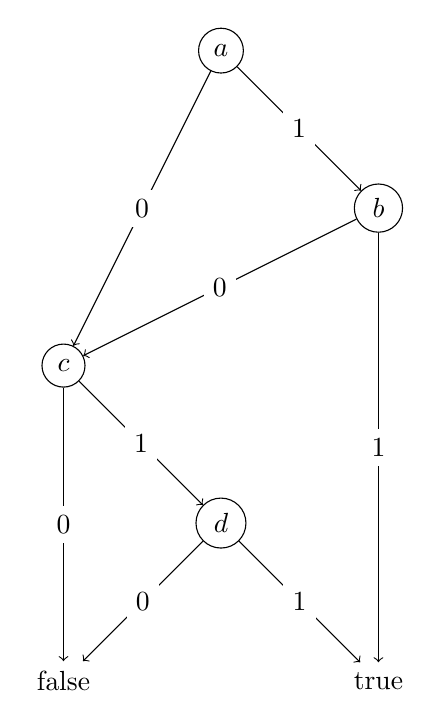
\begin{tikzpicture}[align=center, xscale=2, yscale=2]

\node [circle, draw] (a) at (0, 2) {$a$};
\node [circle, draw] (b) at (1, 1) {$b$};
\node [circle, draw] (c) at (-1, 0) {$c$};
\node [circle, draw] (d) at (0, -1) {$d$};
\node (false) at (-1, -2) {false};
\node (true) at (1, -2) {true};

\draw [->] (a) -- (b) node [midway, fill=white] {1};
\draw [->] (a) -- (c) node [midway, fill=white] {0};
\draw [->] (b) -- (c) node [midway, fill=white] {0};
\draw [->] (b) -- (true) node [midway, fill=white] {1};
\draw [->] (c) -- (false) node [midway, fill=white] {0};
\draw [->] (c) -- (d) node [midway, fill=white] {1};
\draw [->] (d) -- (false) node [midway, fill=white] {0};
\draw [->] (d) -- (true) node [midway, fill=white] {1};

\end{tikzpicture}

\caption{Binary decision diagram for $asdf$}
\label{fig:bdd}

\end{figure}

\paragraph{Data-flow analysis}

\paragraph{Symbolic execution}

\paragraph{Abstract interpretation}


\section{Abstract interpretation}

The abstract interpretation falls into the category of software
verification by static analysis.


\chapter{Solution design}
\label{chap:design}


\section{Prefix}


\section{Suffix}


\section{Trie}


\chapter{Implementation}
\label{chap:implementation}


\chapter{Conclusion}
\label{chap:conclusion}


%% Lists of tables and figures, glossary, etc.
%\printindex
%\printglossary
%\listoffigures
%\listoftables

%% Bibliography
\begin{thebibliography}{99}

\bibitem{CousotCousot77-1}
P{.} Cousot and R{.}Cousot.
\newblock Abstract interpretation: a unified lattice model for static
  analysis of programs by construction or approximation of fixpoints.
\newblock In \emph{Conference Record of the Fourth Annual ACM
  SIGPLAN-SIGACT Symposium on Principles of Programming Languages},
  pages 238--252, Los Angeles, California, 1977. ACM Press, New York,
  NY, USA.

\bibitem{Cousot00-1}
P{.} Cousot.
\newblock Abstract interpretation based formal methods and future
  challenges.
\newblock In \emph{Informatics - 10 Years Back, 10 Years Ahead},
  volume 2000 of LNCS, pages 138--156. Springer, 2000.

\bibitem{Moore65-1}
G{.} E{.} Moore.
\newblock Cramming more components onto integrated circuits.
\newblock In \emph{Electronics}, volume 38, number 8, pages 114--117. 1965.

\bibitem{EmanuelssonNilsson08-1}
P{.} Emanuelsson, U{.} Nilsson.
\newblock A comparative study of industrial static analysis tools (extended
  version).
\newblock In \emph{Electronic Notes in Theoretical Computer Science},
  volume 217, pages 5--21. 2008.

\bibitem{Boulanger12-1}
J{.}--L{.} Boulanger.
\newblock Static Analysis of Software: The Abstract Interpretation.
\newblock Wiley, 2012.

\bibitem{Ernst03-1}
M{.} D{.} Ernst.
\newblock Static and dynamic analysis: Synergy and duality.
\newblock In \emph{Workshop on Dynamic Analysis}, pages 24--27. 2003.

\bibitem{Woodcock09-1}
J{.} Woodcock, P{.} G{.} Larsen, J{.} Bicarregui and J{.} S{.} Fitzgerald.
\newblock Formal methods: Practise and experience.
\newblock In \emph{ACM Computing Surveys}. 2009.

\bibitem{Turing36-1}
A{.} Turing.
\newblock On computable numbers, with an application to the
  Entscheidungsproblem.
\newblock In \emph{Proceedings of the London Mathematical Society},
  pages 230--265. 1936.

\bibitem{Sipser06-1}
M{.} Sipser.
\newblock Introduction to the Theory of Computation (Second Edition).
\newblock Thomson Course Technology, 2006.

\bibitem{Kozen97-1}
D{.} Kozen.
\newblock Automata and Computability.
\newblock Springer, 1997.

\bibitem{Chess04-1}
B{.} Chess, G{.} McGraw.
\newblock Static Analysis for Security.
\newblock In \emph{Security and Privacy, IEEE}, volume 2, number 6,
  pages 76--79, 2004.

\end{thebibliography}


%% Additional materials
\appendix

\chapter{Instructions for running \texttt{canal}}
\label{chap:instructions}

%% End of the whole document
\end{document}

